%----------------------------------------------------------------------------------------
%	TODO LIST
%----------------------------------------------------------------------------------------

% DONE:
% - Backup slide: Asymptotische Komplexität
% - Logo obere linke Ecke auf erster und letzter Folie
% - Hintergrund auf erster und letzter Folie
% - Logo obere rechte Ecke auf Content-Folien

%----------------------------------------------------------------------------------------
%	PACKAGES AND THEMES
%----------------------------------------------------------------------------------------
\documentclass[aspectratio=169,xcolor=dvipsnames, t]{beamer}
\usepackage{fontspec} % Allows using custom font. MUST be before loading the theme!
\usetheme{SimplePlusAIC}
\usepackage{hyperref}
\usepackage{graphicx} % Allows including images
\usepackage{booktabs} % Allows the use of \toprule, \midrule and  \bottomrule in tables
\usepackage{svg} %allows using svg figures
\usepackage{tikz}
\usepackage{makecell}
\usepackage{wrapfig}
% ADD YOUR PACKAGES BELOW

%----------------------------------------------------------------------------------------
%	TITLE PAGE CONFIGURATION
%----------------------------------------------------------------------------------------

\title[Wiring Assistant]{Wiring Assistant} % The short title appears at the bottom of every slide, the full title is only on the title page
\subtitle{Selected Fun Problems of the ACM Programming Contest}

\author{Samuel Füßinger}
\institute[University of Tübingen, Department of Computer Science,
Database Systems]{Database Systems\newline Department of Computer Science
\newline
University of Tübingen
}
% Your institution as it will appear on the bottom of every slide, maybe shorthand to save space


\date{\hfill\hspace{10em}21.06.2024} % Date, can be changed to a custom date


%----------------------------------------------------------------------------------------
%	Custom definitions and stuff
%----------------------------------------------------------------------------------------

\usepackage{mathtools}
\usetikzlibrary{calc}
\usetikzlibrary{backgrounds}
\usepackage{multirow}
\usepackage{appendixnumberbeamer}


% % blue version
% \definecolor{color_circb_bg}{rgb}{0.0, 0.3, 0.5}
% \definecolor{color_circb_grid}{rgb}{0.0, 0.45, 0.75}
% \definecolor{color_circb_wire}{rgb}{0.0, 0.76, 0.92}

% green version
\definecolor{color_circb_bg}{HTML}{053620}
\definecolor{color_circb_grid}{HTML}{2d7454}
\definecolor{color_circb_wire}{HTML}{88c441}
\definecolor{color_circb_wire_highlight}{HTML}{00cfff}
\definecolor{color_circb_metal}{HTML}{e2b677}
\definecolor{color_marker_x}{HTML}{990099}
% \definecolor{color_marker_y}{HTML}{500050}
\colorlet{color_marker_y}{color_marker_x}
\definecolor{color_x_coords}{HTML}{aa0000}
\definecolor{color_y_coords}{HTML}{0000aa}
\definecolor{color_bounds}{HTML}{006437}
% \colorlet{color_bounds}{color_circb_bg}


\def\circbwirelinewidth{1mm}

% \def\circbwire{\@ifnextchar[{\@circbwire}{\@circbwire[color_circb_wire]}} % doesn't work :(
\def\circbwire<#1>[#2](#3,#4,#5,#6){
    \draw<#1>[#2,line width=\circbwirelinewidth] (#3,#4) -- (#5,#6);
    \fill<#1>[#2] (#3,#4) circle (1.5mm);
    \fill<#1>[#2] (#5,#6) circle (1.5mm);
    \begin{pgfonlayer}{metallayer}
        \fill<#1>[color_circb_metal] (#3,#4) circle (1mm);
        \fill<#1>[color_circb_metal] (#5,#6) circle (1mm);
    \end{pgfonlayer}
}

% for consistent placement
\def\reservedspace{\fill[transparent] (-1,-0.5) rectangle (10.5,11.7);}
\newcommand{\graphicoffset}{\vspace{-20mm}\hspace{-2mm}}


\newcommand{\footnotestar}[1]{%
    \begingroup
    \renewcommand{\thefootnote}{\fnsymbol{footnote}}%
    \footnote{#1}%
    \endgroup
}
\setcounter{footnote}{1}%

%----------------------------------------------------------------------------------------
%	PRESENTATION SLIDES
%----------------------------------------------------------------------------------------

\begin{document}




\maketitlepage
\setcounter{framenumber}{0} % Exclude title page from frame number count

% \begin{frame}[t]{Overview}
%     % Throughout your presentation, if you choose to use \section{} and \subsection{} commands, these will automatically be printed on this slide as an overview of your presentation
%     \tableofcontents
% \end{frame}

\begin{frame}{The Task}
    \begin{wrapfigure}{r}{0.48\textwidth}
        \graphicoffset
        \centering
        \begin{tikzpicture}[scale=0.6]
            \reservedspace
            \fill[color_circb_bg, rounded corners=0.75mm] (-0.5,-0.5) rectangle (10.5,10.5);
            \draw[step=1.0,color_circb_grid,line width=0.1mm] (0,0) grid (10,10);
            \pgfdeclarelayer{metallayer}
            \pgfsetlayers{main,metallayer}
            \circbwire<1->[color_circb_wire](5, 0, 5, 6)
            \circbwire<1->[color_circb_wire](0, 5, 6, 5)
            \circbwire<1->[color_circb_wire](9, 1, 9, 6)
            \circbwire<1->[color_circb_wire](7, 4, 7, 7)
            \circbwire<1->[color_circb_wire](8, 6, 8, 8)
            \circbwire<1->[color_circb_wire](4, 6, 6, 6)
            \circbwire<1->[color_circb_wire](8, 8, 10, 8)
            % the points to connect
            \fill<2->[color_circb_wire_highlight] (7,8) circle (1.7mm);
            \fill<2->[color_circb_wire_highlight] (6,1) circle (1.7mm);
            \begin{pgfonlayer}{metallayer}
                \fill<2->[color_circb_metal] (7,8) circle (1mm);
                \fill<2->[color_circb_metal] (6,1) circle (1mm);
            \end{pgfonlayer}
            \draw<3>[color_circb_wire_highlight, line width=\circbwirelinewidth] (7,8) -- (7,1) -- (6,1);
            \draw<3>[red, line width=0.5mm] (6.4,4.9) -- (7.6,6.1);
            \draw<3>[red, line width=0.5mm] (6.4,6.1) -- (7.6,4.9);
            \draw<4>[color_circb_wire_highlight, line width=\circbwirelinewidth] (7,8) -- (3,8) -- (3,1) -- (6,1);
            \draw<5>[color_circb_wire_highlight, line width=\circbwirelinewidth] (7,8) -- (6,8) -- (6,1);
            \draw<6>[color_circb_wire_highlight, line width=\circbwirelinewidth] (7,8) -- (7,9) -- (10,9) -- (10,0) -- (6,0) -- (6,1);
        \end{tikzpicture}
        % \caption{Figure caption}
    \end{wrapfigure}
    \ % I have no idea why this solves the problem
    \begin{itemize}
        \item Grid-based circuit board
        \item Some existing wires
        \item Two points to connect
        \item Wires cannot be stacked
        \item Intersections allowed but costly
        \item What is the minimum possible cost?
    \end{itemize}
\end{frame}



\begin{frame}{Input Format}
    \begin{wrapfigure}{r}{0.48\textwidth}
        \graphicoffset
        \centering
        \begin{tikzpicture}[scale=0.6]
            \reservedspace
            \fill[color_circb_bg, rounded corners=0.75mm] (-0.5,-0.5) rectangle (10.5,10.5);
            \draw[step=1.0,color_circb_grid,line width=0.1mm] (0,0) grid (10,10);
            \pgfdeclarelayer{metallayer}
            \pgfsetlayers{main,metallayer}
            \circbwire<1->[color_circb_wire](5, 0, 5, 6)
            \circbwire<1->[color_circb_wire](0, 5, 6, 5)
            \circbwire<1->[color_circb_wire](9, 1, 9, 6)
            \circbwire<1->[color_circb_wire](7, 4, 7, 7)
            \circbwire<1->[color_circb_wire](8, 6, 8, 8)
            \circbwire<1->[color_circb_wire](4, 6, 6, 6)
            \circbwire<1->[color_circb_wire](8, 8, 10, 8)
            % the points to connect
            \fill[color_circb_wire_highlight] (7,8) circle (1.7mm);
            \fill[color_circb_wire_highlight] (6,1) circle (1.7mm);
            \begin{pgfonlayer}{metallayer}
                \fill[color_circb_metal] (7,8) circle (1mm);
                \fill[color_circb_metal] (6,1) circle (1mm);
            \end{pgfonlayer}
        \end{tikzpicture}
        % \caption{Figure caption}
    \end{wrapfigure}
    % \texttt{7 10}\\
    $\underset{\text{M}}{\texttt{7}}\texttt{ }\underset{\text{S}}{\texttt{11}}$ \vspace{0.5\baselineskip} \\
    $\underset{\text{Coordinates of wire end points\hfill}}{\texttt{5 0 5 6 0 5 6 5 9 1 9 6 7 4 7 7 \dots \hspace{0.6em}}}$ \vspace{0.5\baselineskip}\\
    $\underset{\text{Coordinates of points to connect\hfill}}{\texttt{7 8 6 1}\hfill}$ \vspace{2.0\baselineskip}
    \\
    M\phantom{S}\hspace{-1.75mm}$\coloneq$ Number of wires\\
    S\phantom{M}\hspace{-1.75mm}$\coloneq$ Grid size\\
\end{frame}



\begin{frame}{Naive Approach}
    \begin{wrapfigure}{r}{0.48\textwidth}
        \graphicoffset
        \centering
        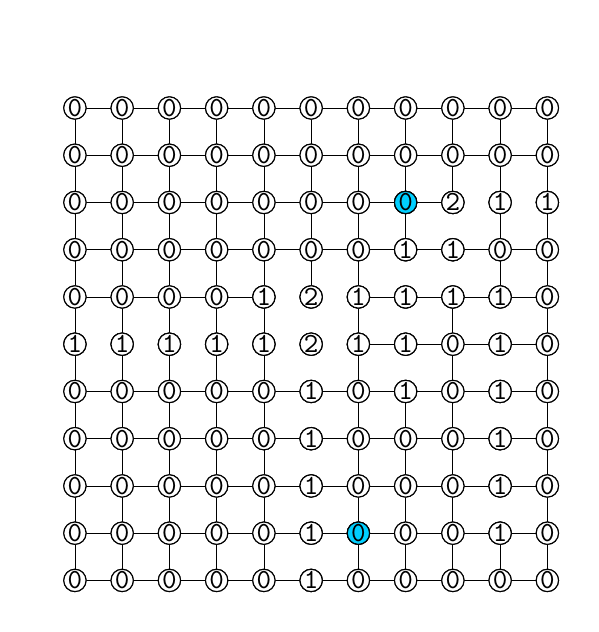
\begin{tikzpicture}[scale=0.6]
            \reservedspace
            \fill[white, rounded corners=0.75mm] (-0.5,-0.5) rectangle (10.5,10.5);
            % \pgfdeclarelayer{metallayer}
            \draw[step=1.0,black,line width=0.1mm] (0,0) grid (10,10);
            % circuit board wire lines
            \draw<1-2>[color_circb_wire, line width=1mm](5, 0) -- (5, 6);
            \draw<1-2>[color_circb_wire, line width=1mm](0, 5) -- (6, 5);
            \draw<1-2>[color_circb_wire, line width=1mm](9, 1) -- (9, 6);
            \draw<1-2>[color_circb_wire, line width=1mm](7, 4) -- (7, 7);
            \draw<1-2>[color_circb_wire, line width=1mm](8, 6) -- (8, 8);
            \draw<1-2>[color_circb_wire, line width=1mm](4, 6) -- (6, 6);
            \draw<1-2>[color_circb_wire, line width=1mm](8, 8) -- (10, 8);
            % eraser lines
            \draw<3->[white, line width=1mm](5, 0) -- (5, 6);
            \draw<3->[white, line width=1mm](0, 5) -- (6, 5);
            \draw<3->[white, line width=1mm](9, 1) -- (9, 6);
            \draw<3->[white, line width=1mm](7, 4) -- (7, 7);
            \draw<3->[white, line width=1mm](8, 6) -- (8, 8);
            \draw<3->[white, line width=1mm](4, 6) -- (6, 6);
            \draw<3->[white, line width=1mm](8, 8) -- (10, 8);
            \foreach \x in {0,1,2,3,4,5,6,7,8,9,10}
                \foreach \y in {0,1,2,3,4,5,6,7,8,9,10}
                    \node<1>[circle,draw, minimum size=2mm, inner sep=0pt, fill=white] at (\x,\y) {\phantom{\texttt{0}}};
            \foreach \x in {0,1,2,3,4,5,6,7,8,9,10}
                \foreach \y in {0,1,2,3,4,5,6,7,8,9,10}
                    \node<2->[circle,draw, minimum size=2mm, inner sep=0pt, fill=white] at (\x,\y) {\texttt{0}};
            % nodes with a non-zero cost:
            \node<2->[circle,draw, minimum size=2mm, inner sep=0pt, fill=white] at (5,0) {\texttt{1}};
            \node<2->[circle,draw, minimum size=2mm, inner sep=0pt, fill=white] at (5,1) {\texttt{1}};
            \node<2->[circle,draw, minimum size=2mm, inner sep=0pt, fill=white] at (5,2) {\texttt{1}};
            \node<2->[circle,draw, minimum size=2mm, inner sep=0pt, fill=white] at (5,3) {\texttt{1}};
            \node<2->[circle,draw, minimum size=2mm, inner sep=0pt, fill=white] at (5,4) {\texttt{1}};
            \node<2->[circle,draw, minimum size=2mm, inner sep=0pt, fill=white] at (5,5) {\texttt{2}};
            \node<2->[circle,draw, minimum size=2mm, inner sep=0pt, fill=white] at (5,6) {\texttt{2}};
            %
            \node<2->[circle,draw, minimum size=2mm, inner sep=0pt, fill=white] at (0,5) {\texttt{1}};
            \node<2->[circle,draw, minimum size=2mm, inner sep=0pt, fill=white] at (1,5) {\texttt{1}};
            \node<2->[circle,draw, minimum size=2mm, inner sep=0pt, fill=white] at (2,5) {\texttt{1}};
            \node<2->[circle,draw, minimum size=2mm, inner sep=0pt, fill=white] at (3,5) {\texttt{1}};
            \node<2->[circle,draw, minimum size=2mm, inner sep=0pt, fill=white] at (4,5) {\texttt{1}};
            % duplicate
            \node<2->[circle,draw, minimum size=2mm, inner sep=0pt, fill=white] at (6,5) {\texttt{1}};
            %
            \node<2->[circle,draw, minimum size=2mm, inner sep=0pt, fill=white] at (9,1) {\texttt{1}};
            \node<2->[circle,draw, minimum size=2mm, inner sep=0pt, fill=white] at (9,2) {\texttt{1}};
            \node<2->[circle,draw, minimum size=2mm, inner sep=0pt, fill=white] at (9,3) {\texttt{1}};
            \node<2->[circle,draw, minimum size=2mm, inner sep=0pt, fill=white] at (9,4) {\texttt{1}};
            \node<2->[circle,draw, minimum size=2mm, inner sep=0pt, fill=white] at (9,5) {\texttt{1}};
            \node<2->[circle,draw, minimum size=2mm, inner sep=0pt, fill=white] at (9,6) {\texttt{1}};
            %
            \node<2->[circle,draw, minimum size=2mm, inner sep=0pt, fill=white] at (7,4) {\texttt{1}};
            \node<2->[circle,draw, minimum size=2mm, inner sep=0pt, fill=white] at (7,5) {\texttt{1}};
            \node<2->[circle,draw, minimum size=2mm, inner sep=0pt, fill=white] at (7,6) {\texttt{1}};
            \node<2->[circle,draw, minimum size=2mm, inner sep=0pt, fill=white] at (7,7) {\texttt{1}};
            %
            \node<2->[circle,draw, minimum size=2mm, inner sep=0pt, fill=white] at (8,6) {\texttt{1}};
            \node<2->[circle,draw, minimum size=2mm, inner sep=0pt, fill=white] at (8,7) {\texttt{1}};
            \node<2->[circle,draw, minimum size=2mm, inner sep=0pt, fill=white] at (8,8) {\texttt{2}};
            %
            \node<2->[circle,draw, minimum size=2mm, inner sep=0pt, fill=white] at (4,6) {\texttt{1}};
            % duplicate
            \node<2->[circle,draw, minimum size=2mm, inner sep=0pt, fill=white] at (6,6) {\texttt{1}};
            %
            % duplicate
            \node<2->[circle,draw, minimum size=2mm, inner sep=0pt, fill=white] at (9,8) {\texttt{1}};
            \node<2->[circle,draw, minimum size=2mm, inner sep=0pt, fill=white] at (10,8) {\texttt{1}};
            % points to connect
            \node<1>[circle,draw, minimum size=2mm, inner sep=0pt, fill=color_circb_wire_highlight] at (7,8) {\phantom{\texttt{0}}};
            \node<1>[circle,draw, minimum size=2mm, inner sep=0pt, fill=color_circb_wire_highlight] at (6,1) {\phantom{\texttt{0}}};
            \node<2->[circle,draw, minimum size=2mm, inner sep=0pt, fill=color_circb_wire_highlight] at (7,8) {\texttt{0}};
            \node<2->[circle,draw, minimum size=2mm, inner sep=0pt, fill=color_circb_wire_highlight] at (6,1) {\texttt{0}};
        \end{tikzpicture}
        % \caption{Figure caption}
    \end{wrapfigure}
    \
    \begin{itemize}
        \item Graph problem
        \item Node cost = Number of wires
        \item Remove edges of existing wires
        \item Use any pathfinding algorithm
    \end{itemize}
\end{frame}


\begin{frame}{Problem}
    \begin{wrapfigure}{r}{0.48\textwidth}
        \graphicoffset
        \centering
        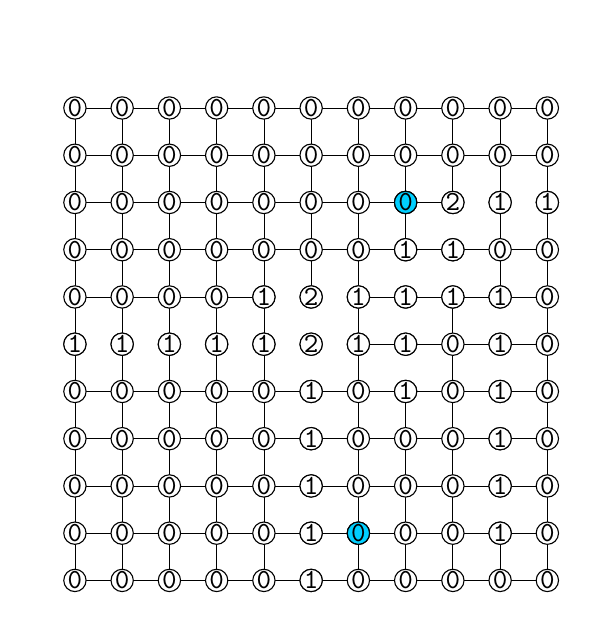
\begin{tikzpicture}[scale=0.6]
            \reservedspace
            \fill[white, rounded corners=0.75mm] (-0.5,-0.5) rectangle (10.5,10.5);
            % \pgfdeclarelayer{metallayer}
            \draw[step=1.0,black,line width=0.1mm] (0,0) grid (10,10);
            % eraser lines
            \draw[white, line width=1mm](5, 0) -- (5, 6);
            \draw[white, line width=1mm](0, 5) -- (6, 5);
            \draw[white, line width=1mm](9, 1) -- (9, 6);
            \draw[white, line width=1mm](7, 4) -- (7, 7);
            \draw[white, line width=1mm](8, 6) -- (8, 8);
            \draw[white, line width=1mm](4, 6) -- (6, 6);
            \draw[white, line width=1mm](8, 8) -- (10, 8);
            
            \foreach \x in {0,1,2,3,4,5,6,7,8,9,10}
                \foreach \y in {0,1,2,3,4,5,6,7,8,9,10}
                    \node[circle,draw, minimum size=2mm, inner sep=0pt, fill=white] at (\x,\y) {\texttt{0}};
            % nodes with a non-zero cost:
            \node[circle,draw, minimum size=2mm, inner sep=0pt, fill=white] at (5,0) {\texttt{1}};
            \node[circle,draw, minimum size=2mm, inner sep=0pt, fill=white] at (5,1) {\texttt{1}};
            \node[circle,draw, minimum size=2mm, inner sep=0pt, fill=white] at (5,2) {\texttt{1}};
            \node[circle,draw, minimum size=2mm, inner sep=0pt, fill=white] at (5,3) {\texttt{1}};
            \node[circle,draw, minimum size=2mm, inner sep=0pt, fill=white] at (5,4) {\texttt{1}};
            \node[circle,draw, minimum size=2mm, inner sep=0pt, fill=white] at (5,5) {\texttt{2}};
            \node[circle,draw, minimum size=2mm, inner sep=0pt, fill=white] at (5,6) {\texttt{2}};
            %
            \node[circle,draw, minimum size=2mm, inner sep=0pt, fill=white] at (0,5) {\texttt{1}};
            \node[circle,draw, minimum size=2mm, inner sep=0pt, fill=white] at (1,5) {\texttt{1}};
            \node[circle,draw, minimum size=2mm, inner sep=0pt, fill=white] at (2,5) {\texttt{1}};
            \node[circle,draw, minimum size=2mm, inner sep=0pt, fill=white] at (3,5) {\texttt{1}};
            \node[circle,draw, minimum size=2mm, inner sep=0pt, fill=white] at (4,5) {\texttt{1}};
            % duplicate
            \node[circle,draw, minimum size=2mm, inner sep=0pt, fill=white] at (6,5) {\texttt{1}};
            %
            \node[circle,draw, minimum size=2mm, inner sep=0pt, fill=white] at (9,1) {\texttt{1}};
            \node[circle,draw, minimum size=2mm, inner sep=0pt, fill=white] at (9,2) {\texttt{1}};
            \node[circle,draw, minimum size=2mm, inner sep=0pt, fill=white] at (9,3) {\texttt{1}};
            \node[circle,draw, minimum size=2mm, inner sep=0pt, fill=white] at (9,4) {\texttt{1}};
            \node[circle,draw, minimum size=2mm, inner sep=0pt, fill=white] at (9,5) {\texttt{1}};
            \node[circle,draw, minimum size=2mm, inner sep=0pt, fill=white] at (9,6) {\texttt{1}};
            %
            \node[circle,draw, minimum size=2mm, inner sep=0pt, fill=white] at (7,4) {\texttt{1}};
            \node[circle,draw, minimum size=2mm, inner sep=0pt, fill=white] at (7,5) {\texttt{1}};
            \node[circle,draw, minimum size=2mm, inner sep=0pt, fill=white] at (7,6) {\texttt{1}};
            \node[circle,draw, minimum size=2mm, inner sep=0pt, fill=white] at (7,7) {\texttt{1}};
            %
            \node[circle,draw, minimum size=2mm, inner sep=0pt, fill=white] at (8,6) {\texttt{1}};
            \node[circle,draw, minimum size=2mm, inner sep=0pt, fill=white] at (8,7) {\texttt{1}};
            \node[circle,draw, minimum size=2mm, inner sep=0pt, fill=white] at (8,8) {\texttt{2}};
            %
            \node[circle,draw, minimum size=2mm, inner sep=0pt, fill=white] at (4,6) {\texttt{1}};
            % duplicate
            \node[circle,draw, minimum size=2mm, inner sep=0pt, fill=white] at (6,6) {\texttt{1}};
            %
            % duplicate
            \node[circle,draw, minimum size=2mm, inner sep=0pt, fill=white] at (9,8) {\texttt{1}};
            \node[circle,draw, minimum size=2mm, inner sep=0pt, fill=white] at (10,8) {\texttt{1}};
            % points to connect
            \node[circle,draw, minimum size=2mm, inner sep=0pt, fill=color_circb_wire_highlight] at (7,8) {\phantom{\texttt{0}}};
            \node[circle,draw, minimum size=2mm, inner sep=0pt, fill=color_circb_wire_highlight] at (6,1) {\phantom{\texttt{0}}};
            \node[circle,draw, minimum size=2mm, inner sep=0pt, fill=color_circb_wire_highlight] at (7,8) {\texttt{0}};
            \node[circle,draw, minimum size=2mm, inner sep=0pt, fill=color_circb_wire_highlight] at (6,1) {\texttt{0}};
        \end{tikzpicture}
        % \caption{Figure caption}
    \end{wrapfigure}
    \
    \begin{itemize}
        \item Big problem: graph size 
        \item Up to $10^9\times10^9$ nodes
        \item Searching through $10^{18}$ nodes could take literal decades!
        \item But $\leq99$ wires
        \item We need to reduce the graph
    \end{itemize}
\end{frame}


% % wrong reduction order
% \begin{frame}{Reduction Idea}
%     \begin{wrapfigure}{r}{0.48\textwidth}
%         \graphicoffset
%         \centering
%         \begin{tikzpicture}[scale=0.6]
%             \reservedspace
%             \fill<1>[color_circb_bg, rounded corners=0.75mm] (-0.5,-0.5) rectangle (10.5,10.5);
%             \fill<2>[color_circb_bg, rounded corners=0.75mm] (-0.5,0.5) rectangle (10.5,10.5);
%             \fill<3>[color_circb_bg, rounded corners=0.75mm] (-0.5,0.5) rectangle (10.5,9.5);
%             \fill<4>[color_circb_bg, rounded corners=0.75mm] (1.5,0.5) rectangle (10.5,9.5);
%             \draw<1>[step=1.0,color_circb_grid,line width=0.1mm] (0,0) grid (10,10);
%             \draw<2>[step=1.0,color_circb_grid,line width=0.1mm] (0,1) grid (10,10);
%             \draw<3>[step=1.0,color_circb_grid,line width=0.1mm] (0,1) grid (10,9);
%             \draw<4>[step=1.0,color_circb_grid,line width=0.1mm] (2,1) grid (10,9);
%             \pgfdeclarelayer{metallayer}
%             \pgfsetlayers{main,metallayer}
%             \circbwire<1>[color_circb_wire](5, 0, 5, 6)
%             \circbwire<2->[color_circb_wire](5, 1, 5, 6)
%             \circbwire<1-3>[color_circb_wire](0, 5, 6, 5)
%             \circbwire<4->[color_circb_wire](2, 5, 6, 5)
%             \circbwire<1>[color_circb_wire](9, 1, 9, 6)
%             \circbwire<2->[color_circb_wire](9, 2, 9, 6)
%             \circbwire<1->[color_circb_wire](7, 4, 7, 7)
%             \circbwire<1->[color_circb_wire](8, 6, 8, 8)
%             \circbwire<1->[color_circb_wire](4, 6, 6, 6)
%             \circbwire<1->[color_circb_wire](8, 8, 10, 8)
%             % the points to connect
%             \fill[color_circb_wire_highlight] (7,8) circle (1.7mm);
%             \fill<1>[color_circb_wire_highlight] (6,1) circle (1.7mm);
%             \fill<2->[color_circb_wire_highlight] (6,2) circle (1.7mm);
%             \begin{pgfonlayer}{metallayer}
%                 \fill[color_circb_metal] (7,8) circle (1mm);
%                 \fill<1>[color_circb_metal] (6,1) circle (1mm);
%                 \fill<2->[color_circb_metal] (6,2) circle (1mm);
%             \end{pgfonlayer}
%             % markers
%             \fill<1>[color_marker_y] (-1, 1.8) -- (-0.7, 2) -- (-1, 2.2);
%             \fill<1-3>[color_marker_y] (-1, 2.8) -- (-0.7, 3) -- (-1, 3.2);
%             \fill<4>[color_marker_y] (1, 2.8) -- (1.3, 3) -- (1, 3.2);
            
%             \fill<1-2>[color_marker_y] (-1, 9.8) -- (-0.7, 10) -- (-1, 10.2);
%             \fill<1-3>[color_marker_y] (-1, 8.8) -- (-0.7, 9) -- (-1, 9.2);
%             \fill<4->[color_marker_y] (1, 8.8) -- (1.3, 9) -- (1, 9.2);
            
%             \fill<1-2>[color_marker_x] (0.8, 11) -- (1, 10.7) -- (1.2, 11);
%             \fill<1-2>[color_marker_x] (1.8, 11) -- (2, 10.7) -- (2.2, 11);
%             \fill<1-2>[color_marker_x] (2.8, 11) -- (3, 10.7) -- (3.2, 11);
%             \fill<3>[color_marker_x] (0.8, 10) -- (1, 9.7) -- (1.2, 10);
%             \fill<3>[color_marker_x] (1.8, 10) -- (2, 9.7) -- (2.2, 10);
%             \fill<3->[color_marker_x] (2.8, 10) -- (3, 9.7) -- (3.2, 10);
%         \end{tikzpicture}
%         % \caption{Figure caption}
%     \end{wrapfigure}
%     \ % I have no idea why this solves the problem
%     \begin{itemize}
%         \item Identical neighboring columns/rows
%             % (
%             % 
\begin{tikzpicture}[scale=0.5]\fill[color_marker_x] (-0.2, 0.3) -- (0,0) -- (0.2, 0.3);\end{tikzpicture}
%             % /
%             % 
\begin{tikzpicture}[scale=0.5]\fill[color_marker_y] (-1, 1.8) -- (-0.7, 2) -- (-1, 2.2);\end{tikzpicture}
%             % )
%             have no effect\\
%         $\Rightarrow$ Remove all but one
%         \item Is this good enough?
%     \end{itemize}
% \end{frame}



\begin{frame}{Reduction Idea}
    \begin{wrapfigure}{r}{0.48\textwidth}
        \graphicoffset
        \centering
        \begin{tikzpicture}[scale=0.6]
            \reservedspace
            \fill<1>[color_circb_bg, rounded corners=0.75mm] (-0.5,-0.5) rectangle (10.5,10.5);
            \fill<2-3>[color_circb_bg, rounded corners=0.75mm] (1.5,-0.5) rectangle (10.5,10.5);
            \fill<4-5>[color_circb_bg, rounded corners=0.75mm] (1.5,0.5) rectangle (10.5,10.5);
            \fill<6>[color_circb_bg, rounded corners=0.75mm] (1.5,0.5) rectangle (10.5,9.5);
            \draw<1>[step=1.0,color_circb_grid,line width=0.1mm] (0,0) grid (10,10);
            \draw<2-3>[step=1.0,color_circb_grid,line width=0.1mm] (2,0) grid (10,10);
            \draw<4-5>[step=1.0,color_circb_grid,line width=0.1mm] (2,1) grid (10,10);
            \draw<6>[step=1.0,color_circb_grid,line width=0.1mm] (2,1) grid (10,9);
            \pgfdeclarelayer{metallayer}
            \pgfsetlayers{main,metallayer}
            \circbwire<1-3>[color_circb_wire](5, 0, 5, 6)
            \circbwire<4->[color_circb_wire](5, 1, 5, 6)
            \circbwire<1>[color_circb_wire](0, 5, 6, 5)
            \circbwire<2->[color_circb_wire](2, 5, 6, 5)
            \circbwire<1-3>[color_circb_wire](9, 1, 9, 6)
            \circbwire<4->[color_circb_wire](9, 2, 9, 6)
            \circbwire<1->[color_circb_wire](7, 4, 7, 7)
            \circbwire<1->[color_circb_wire](8, 6, 8, 8)
            \circbwire<1->[color_circb_wire](4, 6, 6, 6)
            \circbwire<1->[color_circb_wire](8, 8, 10, 8)
            % the points to connect
            \fill[color_circb_wire_highlight] (7,8) circle (1.7mm);
            \fill<1-3>[color_circb_wire_highlight] (6,1) circle (1.7mm);
            \fill<4->[color_circb_wire_highlight] (6,2) circle (1.7mm);
            \begin{pgfonlayer}{metallayer}
                \fill[color_circb_metal] (7,8) circle (1mm);
                \fill<1-3>[color_circb_metal] (6,1) circle (1mm);
                \fill<4->[color_circb_metal] (6,2) circle (1mm);
            \end{pgfonlayer}
            % markers
            \fill<3>[color_marker_y] (1, 1.8) -- (1.3, 2) -- (1, 2.2);
            \fill<3-4>[color_marker_y] (1, 2.8) -- (1.3, 3) -- (1, 3.2);
            
            \fill<5>[color_marker_y] (1, 9.8) -- (1.3, 10) -- (1, 10.2);
            \fill<5-6>[color_marker_y] (1, 8.8) -- (1.3, 9) -- (1, 9.2);
            
            \fill<1>[color_marker_x] (0.8, 11) -- (1, 10.7) -- (1.2, 11);
            \fill<1>[color_marker_x] (1.8, 11) -- (2, 10.7) -- (2.2, 11);
            \fill<1-2>[color_marker_x] (2.8, 11) -- (3, 10.7) -- (3.2, 11);
        \end{tikzpicture}
        % \caption{Figure caption}
    \end{wrapfigure}
    \ % I have no idea why this solves the problem
    \begin{itemize}
        \item Identical neighboring columns/rows
            % (
            % 
\begin{tikzpicture}[scale=0.5]\fill[color_marker_x] (-0.2, 0.3) -- (0,0) -- (0.2, 0.3);\end{tikzpicture}
            % /
            % 
\begin{tikzpicture}[scale=0.5]\fill[color_marker_y] (-1, 1.8) -- (-0.7, 2) -- (-1, 2.2);\end{tikzpicture}
            % )
            have no effect\\
        $\Rightarrow$ Remove all but one
        \item How to implement?
        \item Is this good enough?
    \end{itemize}
\end{frame}





\begin{frame}{Reduction Implementation}
    \begin{wrapfigure}{r}{0.48\textwidth}
        \graphicoffset
        \centering
        \begin{tikzpicture}[scale=0.6]
            \reservedspace
            \fill<1-2>[color_circb_bg, rounded corners=0.75mm] (-0.5,-0.5) rectangle (10.5,10.5);
            \fill<3-5>[color_circb_bg, rounded corners=0.75mm] (1.5,-0.5) rectangle (10.5,10.5);
            \fill<6-8>[color_circb_bg, rounded corners=0.75mm] (1.5,0.5) rectangle (10.5,10.5);
            \fill<9->[color_circb_bg, rounded corners=0.75mm] (1.5,0.5) rectangle (10.5,9.5);
            \draw<1-2>[step=1.0,color_circb_grid,line width=0.1mm] (0,0) grid (10,10);
            \draw<3-5>[step=1.0,color_circb_grid,line width=0.1mm] (2,0) grid (10,10);
            \draw<6-8>[step=1.0,color_circb_grid,line width=0.1mm] (2,1) grid (10,10);
            \draw<9->[step=1.0,color_circb_grid,line width=0.1mm] (2,1) grid (10,9);
            \pgfdeclarelayer{metallayer}
            \pgfsetlayers{main,metallayer}
            \circbwire<1-5>[color_circb_wire](5, 0, 5, 6)
            \circbwire<6->[color_circb_wire](5, 1, 5, 6)
            \circbwire<1-2>[color_circb_wire](0, 5, 6, 5)
            \circbwire<3->[color_circb_wire](2, 5, 6, 5)
            \circbwire<1-5>[color_circb_wire](9, 1, 9, 6)
            \circbwire<6->[color_circb_wire](9, 2, 9, 6)
            \circbwire<1->[color_circb_wire](7, 4, 7, 7)
            \circbwire<1->[color_circb_wire](8, 6, 8, 8)
            \circbwire<1->[color_circb_wire](4, 6, 6, 6)
            \circbwire<1->[color_circb_wire](8, 8, 10, 8)
            % the points to connect
            \fill[color_circb_wire_highlight] (7,8) circle (1.7mm);
            \fill<1-5>[color_circb_wire_highlight] (6,1) circle (1.7mm);
            \fill<6->[color_circb_wire_highlight] (6,2) circle (1.7mm);
            \begin{pgfonlayer}{metallayer}
                \fill[color_circb_metal] (7,8) circle (1mm);
                \fill<1-5>[color_circb_metal] (6,1) circle (1mm);
                \fill<6->[color_circb_metal] (6,2) circle (1mm);
            \end{pgfonlayer}
            % % markers
            % \fill<3>[color_marker_y] (1, 1.8) -- (1.3, 2) -- (1, 2.2);
            % \fill<3-4>[color_marker_y] (1, 2.8) -- (1.3, 3) -- (1, 3.2);
            
            % \fill<5>[color_marker_y] (1, 9.8) -- (1.3, 10) -- (1, 10.2);
            % \fill<5-6>[color_marker_y] (1, 8.8) -- (1.3, 9) -- (1, 9.2);
            
            % \fill<1>[color_marker_x] (0.8, 11) -- (1, 10.7) -- (1.2, 11);
            % \fill<1>[color_marker_x] (1.8, 11) -- (2, 10.7) -- (2.2, 11);
            % \fill<1-2>[color_marker_x] (2.8, 11) -- (3, 10.7) -- (3.2, 11);
            \draw<2>[black] (0,10.6)--(0,10.8)--(4,10.8)--(4,10.6);
            \node<2> at (2,11.1) {$+4$};
            \draw<5>[black] (1.4,1)--(1.2,1)--(1.2,4)--(1.4,4);
            \node<5> at (0.6,2.5) {$+3$};
            \draw<8>[black] (1.4,8)--(1.2,8)--(1.2,11)--(1.4,11);
            \node<8> at (0.6,9.5) {$+3$};
        \end{tikzpicture}
        % \caption{Figure caption}
    \end{wrapfigure}
    \ \vspace{-10mm}\\
    $\underset{\text{Coordinates of wire end points\hfill}}{\texttt{\color{color_x_coords}5 \color{color_y_coords}0 \color{color_x_coords}5 \color{color_y_coords}6 \color{color_x_coords}0 \color{color_y_coords}5 \color{color_x_coords}6 \color{color_y_coords}5 \color{color_x_coords}9 \color{color_y_coords}1 \color{color_x_coords}9 \color{color_y_coords}6 \color{color_x_coords}7 \color{color_y_coords}4 \color{color_x_coords}7 \color{color_y_coords}7 \color{black}\dots \hspace{0.6em}}}$ \vspace{0.5\baselineskip}\\
    $\underset{\text{Coordinates of points to connect\hfill}}{\texttt{\color{color_x_coords}7 \color{color_y_coords}8 \color{color_x_coords}6 \color{color_y_coords}1}\hfill}$ \vspace{1.0\baselineskip}
    \\
    Split into arrays, include {\color{color_bounds}bounds} and sort:\\
    {\only<1-3>{\texttt{\color{color_x_coords}xs = [\color{color_bounds}-1\color{color_x_coords}, 0, 4, 5, 5, 6, 6, 6, 7,}}}
    {\only<4->{\texttt{\color{color_x_coords}xs = [\color{color_bounds}-1\color{color_x_coords}, 0, 2, 3, 3, 4, 4, 4, 5,}}}
    \vspace{-1.5mm}\\
    {\only<2-3>{\phantom{\texttt{-}}\tiny\hspace{18.25mm}$\overset{\begin{tikzpicture}[scale=0.5]\draw[black] (0,0.15)--(0, 0)--(1.65,0)--(1.65,0.15);\end{tikzpicture}}{+4}$}}
    \ \\
    {\only<1-3>{\texttt{\phantom{xs = [}\color{color_x_coords}7, 7, 8, 8, 9, 9, 10, \color{color_bounds}11\color{color_x_coords}]}}}
    {\only<4->{\texttt{\phantom{xs = [}\color{color_x_coords}5, 5, 6, 6, 7, 7, 8, \color{color_bounds}9\color{color_x_coords}]}}}
    \vspace{-1.5mm}\\
    \ \\
    {\only<1-6>{\texttt{\color{color_y_coords}ys = [\color{color_bounds}-1\color{color_y_coords}, 0, 1, 1, 4, 5, 5, 6, 6,}}}
    {\only<7->{\texttt{\color{color_y_coords}ys = [\color{color_bounds}-1\color{color_y_coords}, 0, 1, 1, 3, 4, 4, 5, 5,}}}
    \vspace{-1.5mm}\\
    {\only<5-6>{\phantom{\texttt{-x, x, }}\tiny\hspace{18.25mm}$\overset{\begin{tikzpicture}[scale=0.5]\draw[black] (0,0.15)--(0, 0)--(1.65,0)--(1.65,0.15);\end{tikzpicture}}{+3}$}}
    \ \\
    {\only<1-6>{\texttt{\phantom{ys = [}\color{color_y_coords}6, 6, 6, 7, 8, 8, 8, \color{color_bounds}11\color{color_y_coords}]}}}
    {\only<7-9>{\texttt{\phantom{ys = [}\color{color_y_coords}5, 5, 5, 6, 7, 7, 7, \color{color_bounds}10\color{color_y_coords}]}}}
    {\only<10->{\texttt{\phantom{ys = [}\color{color_y_coords}5, 5, 5, 6, 7, 7, 7, \color{color_bounds}9\color{color_y_coords}]}}}
    \vspace{-1.5mm}\\
    {\only<8-9>{\phantom{\texttt{x, x, x, x, x, }}\tiny\hspace{18.25mm}$\overset{\begin{tikzpicture}[scale=0.5]\draw[black] (0,0.15)--(0, 0)--(2,0)--(2,0.15);\end{tikzpicture}}{+3}$}}
    \ \\
    Search for gaps $\geq3$
\end{frame}



\begin{frame}{Worst Case}
    \begin{wrapfigure}{r}{0.48\textwidth}
        \graphicoffset
        \centering
        \begin{tikzpicture}[scale=0.6]
            \reservedspace
            \fill[color_circb_bg, rounded corners=0.75mm] (-0.5,-0.5) rectangle (10.5,10.5);
            \draw[step=1.0,color_circb_grid,line width=0.1mm] (0,0) grid (10,10);
            \pgfdeclarelayer{metallayer}
            \pgfsetlayers{main,metallayer}
            \circbwire<1->[color_circb_wire](1,1,1,3)
            \circbwire<1->[color_circb_wire](5,7,7,7)
            % the points to connect
            \fill[color_circb_wire_highlight] (3,5) circle (1.7mm);
            \fill[color_circb_wire_highlight] (9,9) circle (1.7mm);
            \begin{pgfonlayer}{metallayer}
                \fill[color_circb_metal] (3,5) circle (1mm);
                \fill[color_circb_metal] (9,9) circle (1mm);
            \end{pgfonlayer}
        \end{tikzpicture}
        % \caption{Figure caption}
    \end{wrapfigure}
    % \texttt{7 10}\\
    Width:\\
    $W = (2\cdot|\textit{unique x-coordinates}|+1)$\\
    \vspace{0.7\baselineskip}
    Height:\\
    $H = (2\cdot|\textit{unique y-coordinates}|+1)$
\end{frame}



\begin{frame}{Worst Case}
    \vspace{-2mm}
    Resulting size: $W\cdot H = (2\cdot|\textit{unique x-coordinates}|+1)\cdot(2\cdot|\textit{unique y-coordinates}|+1)$\\
    \vspace{0.7\baselineskip}
    $\bullet~~$ Up to $99$ wires (up to three unique coordinate components each)\\
    $\bullet~~$ Start and end points (two components each)\\
    $\Rightarrow$ $99\cdot3+2\cdot2=301$ unique components\\
    \vspace{0.7\baselineskip}
    $W+H=(2\cdot|\textit{unique x-coordinates}|+1)+(2\cdot|\textit{unique y-coordinates}|+1)$\\
    $= 2\cdot(|\textit{unique x-coordinates}|+|\textit{unique y-coordinates}|)+2$\\
    $= 2\cdot(|\textit{unique components}|)+2$\\
    $= 2\cdot301+2 = 604$\\
    \vspace{0.7\baselineskip}
    $\Rightarrow$ $W\cdot H\leq\left(\frac{W+H}{2}\right)^2=\left(\frac{604}{2}\right)^2=91204$\\
    $\Rightarrow$ Worst case: $\leq91204$ nodes after reduction
\end{frame}



\begin{frame}{Solution In A Nutshell}
    \begin{wrapfigure}{r}{0.48\textwidth}
        \graphicoffset
        \centering
        \begin{tikzpicture}[scale=0.6]
            \reservedspace
            % -------------------------------------------------------------------
            % PCB
            % -------------------------------------------------------------------
            \fill<1>[color_circb_bg, rounded corners=0.75mm] (-0.5,-0.5) rectangle (10.5,10.5);
            \fill<2>[color_circb_bg, rounded corners=0.75mm] (1.5,0.5) rectangle (10.5,9.5);
            \draw<1>[step=1.0,color_circb_grid,line width=0.1mm] (0,0) grid (10,10);
            \draw<2>[step=1.0,color_circb_grid,line width=0.1mm] (2,1) grid (10,9);
            \pgfdeclarelayer{metallayer}
            \pgfsetlayers{main,metallayer}
            \circbwire<1>[color_circb_wire](5, 0, 5, 6)
            \circbwire<2>[color_circb_wire](5, 1, 5, 6)
            \circbwire<1>[color_circb_wire](0, 5, 6, 5)
            \circbwire<2>[color_circb_wire](2, 5, 6, 5)
            \circbwire<1>[color_circb_wire](9, 1, 9, 6)
            \circbwire<2>[color_circb_wire](9, 2, 9, 6)
            \circbwire<1-2>[color_circb_wire](7, 4, 7, 7)
            \circbwire<1-2>[color_circb_wire](8, 6, 8, 8)
            \circbwire<1-2>[color_circb_wire](4, 6, 6, 6)
            \circbwire<1-2>[color_circb_wire](8, 8, 10, 8)
            % the points to connect
            \fill<1-2>[color_circb_wire_highlight] (7,8) circle (1.7mm);
            \fill<1>[color_circb_wire_highlight] (6,1) circle (1.7mm);
            \fill<2>[color_circb_wire_highlight] (6,2) circle (1.7mm);
            \begin{pgfonlayer}{metallayer}
                \fill<1-2>[color_circb_metal] (7,8) circle (1mm);
                \fill<1>[color_circb_metal] (6,1) circle (1mm);
                \fill<2>[color_circb_metal] (6,2) circle (1mm);
            \end{pgfonlayer}
            % -------------------------------------------------------------------
            % Graph
            % -------------------------------------------------------------------
            \draw<3->[step=1.0,black,line width=0.1mm] (2,1) grid (10,9);
            % eraser lines
            \draw<3->[white, line width=1mm](5, 1) -- (5, 6);
            \draw<3->[white, line width=1mm](2, 5) -- (6, 5);
            \draw<3->[white, line width=1mm](9, 2) -- (9, 6);
            \draw<3->[white, line width=1mm](7, 4) -- (7, 7);
            \draw<3->[white, line width=1mm](8, 6) -- (8, 8);
            \draw<3->[white, line width=1mm](4, 6) -- (6, 6);
            \draw<3->[white, line width=1mm](8, 8) -- (10, 8);

            \begin{pgfonlayer}{metallayer}
                \foreach \x in {2,3,4,5,6,7,8,9,10}
                    \foreach \y in {1,2,3,4,5,6,7,8,9}
                        \node<3->[circle,draw, minimum size=2mm, inner sep=0pt, fill=white] at (\x,\y) {\texttt{0}};
                % nodes with non-zero cost:
                \node<3->[circle,draw, minimum size=2mm, inner sep=0pt, fill=white] at (5,1) {\texttt{1}};
                \node<3->[circle,draw, minimum size=2mm, inner sep=0pt, fill=white] at (5,2) {\texttt{1}};
                \node<3->[circle,draw, minimum size=2mm, inner sep=0pt, fill=white] at (5,3) {\texttt{1}};
                \node<3->[circle,draw, minimum size=2mm, inner sep=0pt, fill=white] at (5,4) {\texttt{1}};
                \node<3->[circle,draw, minimum size=2mm, inner sep=0pt, fill=white] at (5,5) {\texttt{2}};
                \node<3->[circle,draw, minimum size=2mm, inner sep=0pt, fill=white] at (5,6) {\texttt{2}};
                %
                \node<3->[circle,draw, minimum size=2mm, inner sep=0pt, fill=white] at (2,5) {\texttt{1}};
                \node<3->[circle,draw, minimum size=2mm, inner sep=0pt, fill=white] at (3,5) {\texttt{1}};
                \node<3->[circle,draw, minimum size=2mm, inner sep=0pt, fill=white] at (4,5) {\texttt{1}};
                % duplicate
                \node<3->[circle,draw, minimum size=2mm, inner sep=0pt, fill=white] at (6,5) {\texttt{1}};
                %
                \node<3->[circle,draw, minimum size=2mm, inner sep=0pt, fill=white] at (9,2) {\texttt{1}};
                \node<3->[circle,draw, minimum size=2mm, inner sep=0pt, fill=white] at (9,3) {\texttt{1}};
                \node<3->[circle,draw, minimum size=2mm, inner sep=0pt, fill=white] at (9,4) {\texttt{1}};
                \node<3->[circle,draw, minimum size=2mm, inner sep=0pt, fill=white] at (9,5) {\texttt{1}};
                \node<3->[circle,draw, minimum size=2mm, inner sep=0pt, fill=white] at (9,6) {\texttt{1}};
                %
                \node<3->[circle,draw, minimum size=2mm, inner sep=0pt, fill=white] at (7,4) {\texttt{1}};
                \node<3->[circle,draw, minimum size=2mm, inner sep=0pt, fill=white] at (7,5) {\texttt{1}};
                \node<3->[circle,draw, minimum size=2mm, inner sep=0pt, fill=white] at (7,6) {\texttt{1}};
                \node<3->[circle,draw, minimum size=2mm, inner sep=0pt, fill=white] at (7,7) {\texttt{1}};
                %
                \node<3->[circle,draw, minimum size=2mm, inner sep=0pt, fill=white] at (8,6) {\texttt{1}};
                \node<3->[circle,draw, minimum size=2mm, inner sep=0pt, fill=white] at (8,7) {\texttt{1}};
                \node<3->[circle,draw, minimum size=2mm, inner sep=0pt, fill=white] at (8,8) {\texttt{2}};
                %
                \node<3->[circle,draw, minimum size=2mm, inner sep=0pt, fill=white] at (4,6) {\texttt{1}};
                % duplicate
                \node<3->[circle,draw, minimum size=2mm, inner sep=0pt, fill=white] at (6,6) {\texttt{1}};
                %
                % duplicate
                \node<3->[circle,draw, minimum size=2mm, inner sep=0pt, fill=white] at (9,8) {\texttt{1}};
                \node<3->[circle,draw, minimum size=2mm, inner sep=0pt, fill=white] at (10,8) {\texttt{1}};
                % points to connect
                \node<3->[circle,draw, minimum size=2mm, inner sep=0pt, fill=color_circb_wire_highlight] at (7,8) {\texttt{0}};
                \node<3->[circle,draw, minimum size=2mm, inner sep=0pt, fill=color_circb_wire_highlight] at (6,2) {\texttt{0}};
            \end{pgfonlayer}
            % solution path
            \draw<4>[color_circb_wire_highlight, line width=\circbwirelinewidth] (7,8) -- (7,9) -- (10,9) -- (10,1) -- (6,1) -- (6,2);
            \node<4> at (3.75,0.2) {\texttt{result>>> 1}};
        \end{tikzpicture}
        % \caption{Figure caption}
    \end{wrapfigure}
    \ % I have no idea why this solves the problem
    \begin{enumerate}
        \item Parse input
        \item Reduce
        \item Build graph
        \item A$^*$ on graph
    \end{enumerate}
\end{frame}



\begin{frame}{Why C?}
    \begin{columns}[T] % align columns from top
        \begin{column}{0.5\textwidth}
            \begin{itemize}
                \item C is fast
                \item Pointers enable elegant solutions
                \item Personal preference
            \end{itemize}
        \end{column}
        \begin{column}{0.5\textwidth}
            \centering
            \vspace{-8mm}
            \includesvg[width=0.75\linewidth]{AICStyleData/img/C_Programming_Language.svg}
        \end{column}
    \end{columns}
\end{frame}



%----------------------------------------------------------------------------------------
% Final PAGE
%----------------------------------------------------------------------------------------

\finalpagetext{Any Questions?}
\makefinalpage
\setcounter{framenumber}{10} % Exclude final page from framenumber count % TODO: check if this number is still correct



%----------------------------------------------------------------------------------------
% BACKUP SLIDES
%----------------------------------------------------------------------------------------
\appendix
\setbeamertemplate{footline}{%
  \begin{beamercolorbox}[ht=3em,sep=0.75em,wd=\paperwidth,leftskip=0.5cm,rightskip=0.5cm]{footlinecolor}
    \tiny{\insertshortinstitute}
    \hspace{1cm}
    \hfill
    \tiny{Appendix \insertframenumber/\inserttotalframenumber}
  \end{beamercolorbox}%
}




\begin{frame}{Complexity (simplified\footnotestar{see the paper for the exact complexities})}
    For grid size $s$ and number of wires $m$:\\
    {\footnotesize(Ignoring the $\mathrm{log}(s)$-factor for growing number of digits)\\}

    \begin{table}[h!]
        \centering
        \begin{tabular}{|l|c|c|}
            \cline{2-3}
            \multicolumn{1}{c|}{}       & \textbf{Time}                       & \textbf{Space}                    \\ \hline
            \textbf{Parsing}            & $\mathcal O(m)$                     & $\mathcal O(m)$                   \\ \hline
            \textbf{Reduction}          & $\mathcal O(m\log m)$               & $\mathcal O(m)$                   \\ \hline
            \textbf{Building the Graph} & $\mathcal O(|V|)=\mathcal O(m^2)$   & $\mathcal O(|V|)=\mathcal O(m^2)$ \\ \hline
            \textbf{A$\mathbf{^*}$}     & $\mathcal O(|E|\log|V|)=\mathcal O(m^2\log m)$\footnotestar{Because $|E|\approx2|V|$}   & $\mathcal O(|V|)=\mathcal O(m^2)$ \\ \hline
            \hline
            \textbf{Total}              & $\mathcal O(m^2\log m)$             & $\mathcal O(m^2)$                 \\ \hline
        \end{tabular}
        % \caption{Complexity}
        % \label{tab:table_complexity}
    \end{table}
    Basically independent of input grid size $s$!
\end{frame}




\begin{frame}{Worst Case (Time/Space)}
    \begin{wrapfigure}{r}{0.50\textwidth}
    %     \graphicoffset
        \centering
        \vspace{-15mm}
        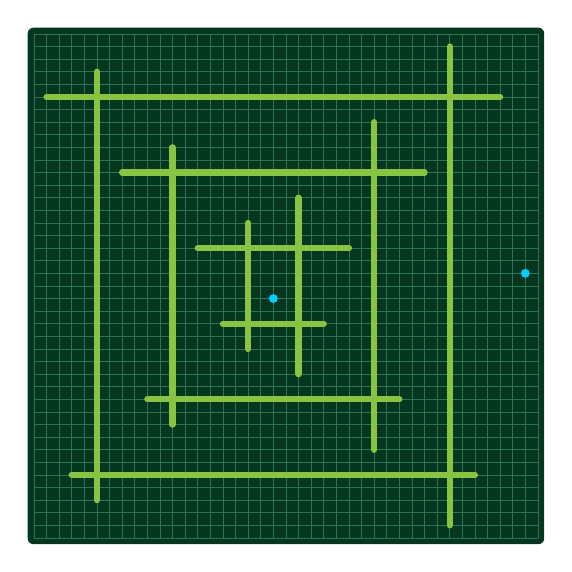
\begin{tikzpicture}[scale=0.16]
            \fill[color_circb_bg, rounded corners=0.75mm] (-0.5,-0.5) rectangle (40.5,40.5);
            \draw[step=1.0,color_circb_grid,line width=0.1mm] (0,0) grid (40,40);
            \pgfdeclarelayer{metallayer}
            \pgfsetlayers{main,metallayer}
            \draw[color_circb_wire, line cap=round, line width=0.8mm](3,5) -- (35,5);
            \draw[color_circb_wire, line cap=round, line width=0.8mm](5,3) -- (5,37);
            \draw[color_circb_wire, line cap=round, line width=0.8mm](1,35) -- (37,35);
            \draw[color_circb_wire, line cap=round, line width=0.8mm](33,1) -- (33,39);
            \draw[color_circb_wire, line cap=round, line width=0.8mm](9,11) -- (29,11);
            \draw[color_circb_wire, line cap=round, line width=0.8mm](7,29) -- (31,29);
            \draw[color_circb_wire, line cap=round, line width=0.8mm](11,9) -- (11,31);
            \draw[color_circb_wire, line cap=round, line width=0.8mm](27,7) -- (27,33);
            \draw[color_circb_wire, line cap=round, line width=0.8mm](15,17) -- (23,17);
            \draw[color_circb_wire, line cap=round, line width=0.8mm](13,23) -- (25,23);
            \draw[color_circb_wire, line cap=round, line width=0.8mm](17,15) -- (17,25);
            \draw[color_circb_wire, line cap=round, line width=0.8mm](21,13) -- (21,27);

            
            \fill<1>[color_circb_wire_highlight] (19,19) circle (3.5mm);
            \fill<1>[color_circb_wire_highlight] (39,21) circle (3.5mm);
            % \begin{pgfonlayer}{metallayer}
            %     \fill<1->[color_circb_metal] (19,19) circle (1mm);
            %     \fill<1->[color_circb_metal] (39,21) circle (1mm);
            % \end{pgfonlayer}
        \end{tikzpicture}
        % \caption{Figure caption}
    \end{wrapfigure}
    Explanatory simplification\\ with fewer cables
\end{frame}




\begin{frame}{Worst Case (Cost)}
    \begin{wrapfigure}{r}{0.50\textwidth}
    %     \graphicoffset
        \centering
        \vspace{-15mm}
        \begin{tikzpicture}[scale=0.6]
            \fill[color_circb_bg, rounded corners=0.75mm] (-0.5,-0.5) rectangle (10.5,10.5);
            \draw[step=1.0,color_circb_grid,line width=0.1mm] (0,0) grid (10,10);
            \pgfdeclarelayer{metallayer}
            \pgfsetlayers{main,metallayer}
            \circbwire<1->[color_circb_wire](0,1,10,1)
            \circbwire<1->[color_circb_wire](0,2,10,2)
            \circbwire<1->[color_circb_wire](0,3,10,3)
            \circbwire<1->[color_circb_wire](0,4,10,4)
            \circbwire<1->[color_circb_wire](0,5,10,5)
            \circbwire<1->[color_circb_wire](0,6,10,6)
            \circbwire<1->[color_circb_wire](0,7,10,7)
            \circbwire<1->[color_circb_wire](0,8,10,8)
            \circbwire<1->[color_circb_wire](0,9,10,9)

            \circbwire<1->[color_circb_wire](0,0,1,0)
            \circbwire<1->[color_circb_wire](1,10,2,10)
            \circbwire<1->[color_circb_wire](2,0,3,0)
            \circbwire<1->[color_circb_wire](3,10,4,10)
            \circbwire<1->[color_circb_wire](4,0,5,0)
            \circbwire<1->[color_circb_wire](5,10,6,10)
            \circbwire<1->[color_circb_wire](6,0,7,0)
            \circbwire<1->[color_circb_wire](7,10,8,10)
            \circbwire<1->[color_circb_wire](8,0,9,0)
            \circbwire<1->[color_circb_wire](9,10,10,10)
            
            % the points to connect
            \fill<1->[color_circb_wire_highlight] (0,0) circle (2.5mm);
            \fill<1->[color_circb_wire_highlight] (10,10) circle (2.5mm);
            \begin{pgfonlayer}{metallayer}
                \fill<1->[color_circb_metal] (0,0) circle (1mm);
                \fill<1->[color_circb_metal] (10,10) circle (1mm);
            \end{pgfonlayer}
        \end{tikzpicture}
        % \caption{Figure caption}
    \end{wrapfigure}
    Explanatory simplification\\ with fewer cables
\end{frame}




\end{document}
